\let\negmedspace\undefined
\let\negthickspace\undefined
\documentclass[journal]{IEEEtran}
\usepackage[a5paper, margin=10mm, onecolumn]{geometry}
\usepackage{lmodern} % Ensure lmodern is loaded for pdflatex
\usepackage{tfrupee} % Include tfrupee package

\setlength{\headheight}{1cm} % Set the height of the header box
\setlength{\headsep}{0mm}     % Set the distance between the header box and the top of the text

\usepackage{gvv-book}
\usepackage{gvv}
\usepackage{cite}
\usepackage{amsmath,amssymb,amsfonts,amsthm}
\usepackage{algorithmic}
\usepackage{graphicx}
\usepackage{textcomp}
\usepackage{xcolor}
\usepackage{txfonts}
\usepackage{listings}
\usepackage{enumitem}
\usepackage{mathtools}
\usepackage{gensymb}
\usepackage{comment}
\usepackage[breaklinks=true]{hyperref}
\usepackage{tkz-euclide} 
\usepackage{listings}
\usepackage{gvv}                                        
\def\inputGnumericTable{}                                 
\usepackage[latin1]{inputenc}                                
\usepackage{color}                                            
\usepackage{array}                                            
\usepackage{longtable}                                       
\usepackage{calc}                                             
\usepackage{multirow}                                         
\usepackage{hhline}                                           
\usepackage{ifthen}                                           
\usepackage{lscape}
\begin{document}

\bibliographystyle{IEEEtran}
\vspace{3cm}

\title{12.8.3.10}
\author{EE24BTECH11060-Sruthi bijili}
% \maketitle
% \newpage
% \bigskip
{\let\newpage\relax\maketitle}
\textbf{Question:}\\
Find the area enclosed by the parabola $x^2=y$ and the line $y=x+2$ and the x-axis.

\solution\\

The equation of parabola is $g \brak{\vec{x}} = \vec{x}^{\top}\vec{V}\vec{x} + 2 \vec{u}^{\top}\vec{x} + f = 0$. In matrix form, it is given by,
\begin{align}
	\myvec{x & y} \myvec{1 & 0 \\ 0 & 0} \myvec{x \\ y} + 2 \myvec{0 & -\frac{1}{2}} \myvec{x \\ y} + 0 = 0
\end{align}
Line equation is,
\begin{align}
	\vec{x} = \kappa \myvec{1 \\ 1} + \myvec{0 \\ 2}
\end{align}
Intersection of a line and a conic is given by,
\begin{align}
	\kappa_i = \frac{-\vec{m}^{\top}\brak{\vec{Vh}+\vec{u}}\pm\sqrt{\sbrak{\vec{m}^{\top}\brak{\vec{Vh}+\vec{u}}}^2-g\brak{h}\brak{\vec{m}^{\top}\vec{Vm}}}}{\vec{m}^{\top}\vec{Vm}}
\end{align}
For the given conic, $\vec{V}=\myvec{1 & 0 \\ 0 & 0 }, \vec{u} = \myvec{0 \\ -\frac{1}{2}}, f = 0$. For the given line, $\vec{h}=\myvec{0 \\ 2}$, $\vec{m}=\myvec{1 \\ 1}$
\begin{multline}
     k_i =\frac{1}{\myvec{1 
 & 1}\myvec{1 &0  \\ 0 & 0}\myvec{1 \\ 1}}\brak{-\myvec{1&1}\brak{\myvec{1&0\\0&0}\myvec{0\\2}+\myvec{0\\ -\frac{1}{2}}}}\pm \\
     \sqrt{\sbrak{\myvec{1&1}\brak{\myvec{1&0\\0&0}\myvec{0\\2}+\myvec{0\\-\frac{1}{2}}}}^2-g\brak{h}\brak{\myvec{1&1}\myvec{1&0\\0&0}\myvec{1\\1}}} 
\end{multline}
by the solving the equation we get
\begin{align}	
	\implies \kappa_i = \myvec{ 2\\4} , \myvec{-1\\ 1}
\end{align}
The 2 curves meet at the points \myvec{2\\4} and \myvec{-1\\ 1}. So, the area between the curves is given by,\\
\textbf{Theoretical Solution:}\\
\begin{align}
	\int{\brak{x + 2} - {\brak{x^2}}}
\end{align}



\begin{align}
	\int{\brak{x + 2} - {\brak{x^2}}} \\
	= \sbrak{{\frac{x^2}{2}} + 2x}_{-1}^{2} - \sbrak{{\frac{x^3}{3}}}_{-1}^{2}\\
	= \brak{\frac{15}{2}} - \brak{3}\\
	= \frac{9}{2} sq.units
\end{align}

\textbf{Simulated Solution:}\\
Using the Trapezoidal rule which approximates the integral of a function $f\brak{x}$ over an interval $\sbrak{a,b}$ by dividing the interval into $n$ subintervals and approximating the area under the curve as a series of trapezoids
\begin{align}
    \int_a^b f\brak{x}dx\approx\frac{h}{2}\sbrak{f\brak{x_0}+2\sum_{i=1}^{n-1}\brak{f\brak{x_i}+f\brak{x_n}}}
\end{align}
Where $x_0$ is semi-major axis of ellipse and $x_n$ is semi-minor axis of the ellipse and $h$ is the width of each subinterval.
\begin{align}
    x_n=x_0+n\cdot h\\
    \implies h=\frac{x_n-x_0}{n}
\end{align}
Using this equation we can get the total area under the cuve by taking the sum of $A_1$ to $A_n$.\\
\begin{align}
	A &= \frac{1}{2} h \brak{y \brak{x_1} + y \brak{x_0}}+ \frac{1}{2} h \brak{y \brak{x_2} + y \brak{x_1}} + \dots + \frac{1}{2} h \brak{y \brak{x_n} + y\brak{x_{n-1}}}\\
	&= h \sbrak{\frac{1}{2} \brak{y \brak{x_0} + y \brak{x_n}} + y \brak{x_1} + \dots + y \brak{x_{n-1}}}
\end{align}
By the first principle of derivatives,\\
\begin{align}
	y\brak{x+h} = y\brak{x} + h y^{\prime}\brak{x}
\end{align}
In this case, to calculate the area enclosed between the line and the parabola, we subtract the $y$ coordinate of the parabola from the $y$ coordinate of the line and then apply the trapezoidal rule on that function.\\
For the parabola,
\begin{align}
	\frac{dy}{dx} = 2x
\end{align}
For the line,
\begin{align}
	\frac{dy}{dx} = 1
\end{align}
The general area element in this case is given by,
\begin{align}
	A_n &= \frac{1}{2} h \brak{y\brak{x_n} + \brak{y\brak{x_n} + hy^\prime\brak{x_n}}} - \frac{1}{2} h \brak{y\brak{x_n} + \brak{y\brak{x_n} + hy^\prime\brak{x_n}}}\\
	A_n &= \frac{1}{2} h \brak{x_n + 2 + h - x_n^2 - h2x}\\
\end{align}
The general difference equation is given by,
\begin{align}
	A_{n+1} &= A_n + \frac{1}{2}h\brak{x_n + 2 + h - x_n^2 - h2x}\\
	x_{n+1} &= x_n + h
\end{align}
By iterating through the required value of $n$, we get the area enclosed between the line and the parabola.\\
Theoretical area $= \frac{9}{2}$ sq.units\\
Calculated area through trapezoidal rule $=4.21875$ sq.units\\

Below is the plot for line and the parabola
\begin{figure}[h!]
	\centering
	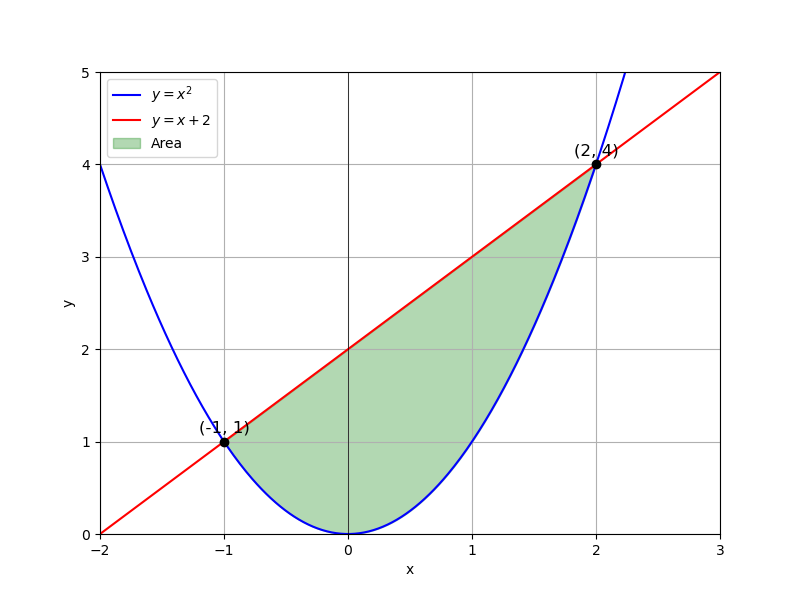
\includegraphics[width=1\columnwidth]{figs/fig.png}
	\label{stemplot}
\end{figure}

\end{document}
